% Options for packages loaded elsewhere
\PassOptionsToPackage{unicode}{hyperref}
\PassOptionsToPackage{hyphens}{url}
\PassOptionsToPackage{dvipsnames,svgnames*,x11names*}{xcolor}
%
\documentclass[
]{article}
\usepackage{lmodern}
\usepackage{amssymb,amsmath}
\usepackage{ifxetex,ifluatex}
\ifnum 0\ifxetex 1\fi\ifluatex 1\fi=0 % if pdftex
  \usepackage[T1]{fontenc}
  \usepackage[utf8]{inputenc}
  \usepackage{textcomp} % provide euro and other symbols
\else % if luatex or xetex
  \usepackage{unicode-math}
  \defaultfontfeatures{Scale=MatchLowercase}
  \defaultfontfeatures[\rmfamily]{Ligatures=TeX,Scale=1}
\fi
% Use upquote if available, for straight quotes in verbatim environments
\IfFileExists{upquote.sty}{\usepackage{upquote}}{}
\IfFileExists{microtype.sty}{% use microtype if available
  \usepackage[]{microtype}
  \UseMicrotypeSet[protrusion]{basicmath} % disable protrusion for tt fonts
}{}
\makeatletter
\@ifundefined{KOMAClassName}{% if non-KOMA class
  \IfFileExists{parskip.sty}{%
    \usepackage{parskip}
  }{% else
    \setlength{\parindent}{0pt}
    \setlength{\parskip}{6pt plus 2pt minus 1pt}}
}{% if KOMA class
  \KOMAoptions{parskip=half}}
\makeatother
\usepackage{xcolor}
\IfFileExists{xurl.sty}{\usepackage{xurl}}{} % add URL line breaks if available
\IfFileExists{bookmark.sty}{\usepackage{bookmark}}{\usepackage{hyperref}}
\hypersetup{
  colorlinks=true,
  linkcolor=blue,
  filecolor=Maroon,
  citecolor=Blue,
  urlcolor=Blue,
  pdfcreator={LaTeX via pandoc}}
\urlstyle{same} % disable monospaced font for URLs
\usepackage{graphicx}
\makeatletter
\def\maxwidth{\ifdim\Gin@nat@width>\linewidth\linewidth\else\Gin@nat@width\fi}
\def\maxheight{\ifdim\Gin@nat@height>\textheight\textheight\else\Gin@nat@height\fi}
\makeatother
% Scale images if necessary, so that they will not overflow the page
% margins by default, and it is still possible to overwrite the defaults
% using explicit options in \includegraphics[width, height, ...]{}
\setkeys{Gin}{width=\maxwidth,height=\maxheight,keepaspectratio}
% Set default figure placement to htbp
\makeatletter
\def\fps@figure{htbp}
\makeatother
\setlength{\emergencystretch}{3em} % prevent overfull lines
\providecommand{\tightlist}{%
  \setlength{\itemsep}{0pt}\setlength{\parskip}{0pt}}
\setcounter{secnumdepth}{-\maxdimen} % remove section numbering
\ifluatex
  \usepackage{selnolig}  % disable illegal ligatures
\fi

\author{}
\date{}

\begin{document}

\newcommand{\Ber}{\operatorname{Ber}}
\newcommand{\E}{\operatorname{E}}
\newcommand{\V}{\operatorname{Var}}
\newcommand{\diag}{\operatorname{diag}}

\newcommand{\bi}{\mathbf{i}}
\newcommand{\bj}{\mathbf{j}}
\newcommand{\bt}{\mathbf{t}}

\newcommand{\bh}{{\boldsymbol{h}}}
\newcommand{\bw}{{\boldsymbol{w}}}
\newcommand{\bv}{{\boldsymbol{v}}}
\newcommand{\bx}{{\boldsymbol{x}}}
\newcommand{\by}{{\boldsymbol{y}}}
\newcommand{\bb}{{\boldsymbol{b}}}
\newcommand{\bz}{{\boldsymbol{z}}}
\newcommand{\bu}{{\boldsymbol{u}}}
\newcommand{\bX}{{\boldsymbol{X}}}
\newcommand{\bY}{{\boldsymbol{Y}}}
\newcommand{\bZ}{{\boldsymbol{Z}}}

\hypertarget{multivariate-gaussian}{%
\section{Multivariate Gaussian}\label{multivariate-gaussian}}

\hypertarget{probabilistic-approach-to-linear-regression}{%
\subsection{Probabilistic Approach to Linear
Regression}\label{probabilistic-approach-to-linear-regression}}

\begin{itemize}
\item
  \(X\): random variable\\
  \(p(x)\): probability density function of \(X\)\\
  \hspace*{0.333em}\hspace*{0.333em} \(\Longleftrightarrow\) ~~
  \(p(x) \ge 0\), ~~ \(\int_{-\infty}^\infty p(x) dx =1\) ~~ and
  \[ P[ a \le X \le b ]= \int_a^b p(x) dx \]
\item
  For example, the \emph{normal} random variable with mean \(\mu\) and
  variance \(\sigma^2\) has the density function
  \[ p(x) = \frac 1 {\sqrt{2 \pi \sigma^2}} \exp \left ( -\tfrac{(x-\mu)^2}{2 \sigma^2} \right ). \]
  In this case, we write \(X \sim \mathcal N (\mu, \sigma^2)\) and
  \[ p(x) = \mathcal N(x| \mu, \sigma^2) .\]
\end{itemize}

\begin{figure}
\hypertarget{fig:normal}{%
\centering
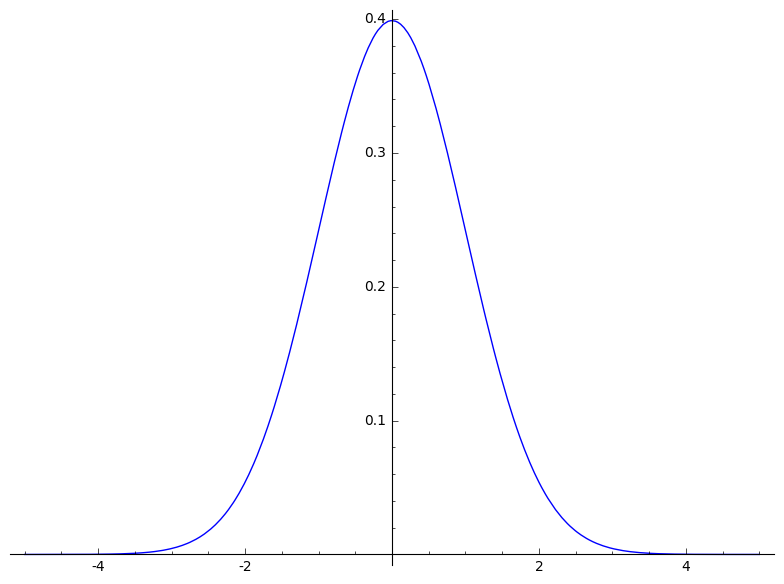
\includegraphics[width=0.5\textwidth,height=\textheight]{normal.png}
\caption{Graph of \(\mathcal N(x|0,1)\)}\label{fig:normal}
}
\end{figure}

\begin{itemize}
\item
  \(X,Y\): two random variables\\
  \(p(x,y)\): (joint) probability density function\\
  \hspace*{0.333em}\hspace*{0.333em}\(\Longleftrightarrow\) ~~
  \(p(x,y) \ge 0\),~~
  \(\int_{-\infty}^\infty \int_{-\infty}^\infty p(x,y) dx dy =1\) ~~ and
  \[ P[ (X,Y) \in A ]= \iint \limits_A p(x,y) dx dy \]
\item
  Marginal density functions:
  \[p_X(x)= \int_{-\infty}^\infty p(x,y) \, dy  \quad\text{ and } \quad p_Y(y)= \int_{-\infty}^\infty p(x,y) \, dx\]
\item
  The \emph{covariance} of \(X\) and \(Y\) is defined by
  \[ \mathrm{Cov}(X,Y)= \operatorname{E}[ (X-\operatorname{E}(X)) (Y-\operatorname{E}(Y))]=\operatorname{E}(XY) -\operatorname{E}(X)\operatorname{E}(Y) .\]
\item
  The \emph{conditional density} of \(X\) given that \(Y=y\) is defined
  to be
  \[ p_{X|Y}(x|y)= \frac {p(x,y)}{p_Y(y)}= \frac {p(x,y)}{\int p(u,y)du} .\]
\item
  More generally, we consider
  \[ T,X_1, \dots, X_m: \text{ random variables}. \] Let
  \({\boldsymbol{x}}=(x_1, \dots , x_m)\). Then we have\\
  \(p(t,{\boldsymbol{x}})\): probability density, ~~\\
  \(p(t|{\boldsymbol{x}})\): conditional density
\item
  Given random variables \(X_1, \dots , X_m\), the \emph{covariance
  matrix} is defined to be \[ \Sigma = [ \mathrm{Cov}(X_i, X_j) ]. \]
\end{itemize}

Recall the settings of linear regression.

\begin{itemize}
\item
  Input: \(x\) ~~ Output: \(t\)\\
  Observations: \((x_1,t_1), (x_2, t_2), \dots , (x_N, t_N)\)
\item
  In many applications we expect some noise in determining the output,
  and the following assumption is reasonable.
\item
  Assume that given \(x\), the corresponding value of \(t\) has a normal
  distribution with a mean equal to the value \(y(x, {\boldsymbol{w}})\)
  of the polynomial curve
  \[ y(x,{\boldsymbol{w}}) = w_0 +w_1 x + w_2 x^2 + \cdots + w_D x^D ,\]
  where \({\boldsymbol{w}}=[w_0, w_1, \dots , w_D]^\top\).
\item
  That is to say,\\
  \[ t=y(x,{\boldsymbol{w}})+\epsilon , \] where \(\epsilon\) is a
  Gaussian noise with variance \(\sigma^2\). Then we can write
  \[ p(t|x, {\boldsymbol{w}}, \beta) = \mathcal N(t|y(x, {\boldsymbol{w}}), \beta^{-1}), \]
  where \(\beta = 1/\sigma^2\) is the inverse variance, called
  \emph{precision}.
\item
  Given \({\boldsymbol{x}}=(x_1, \dots , x_N)\) and
  \(\mathbf{t}= (t_1, \dots , t_N)\), we have
  \[ p(\mathbf{t}|{\boldsymbol{x}}, {\boldsymbol{w}}, \beta) = \prod_{n=1}^N \mathcal N(t_n|y(x_n, {\boldsymbol{w}}), \beta^{-1}). \]
\item
  Let \({\boldsymbol{x}}=(x_1, \dots, x_N)\) and
  \(\mathbf{t}= (t_1,\dots, t_N)\) be given.\\
  \textbf{Task}: Determine \({\boldsymbol{w}}\) and \(\beta\) by maximum
  likelihood.\\
  This is a probabilistic approach to the regression problem.
\item
  We have
\end{itemize}

\[ p(\mathbf{t}|{\boldsymbol{x}}, {\boldsymbol{w}}, \beta) = \prod_{n=1}^N \mathcal N(t_n|y(x_n, {\boldsymbol{w}}), \beta^{-1}). \]

To maximize this function, we take logarithm:
\[ \ln p(\mathbf{t}|{\boldsymbol{x}}, {\boldsymbol{w}}, \beta) = -\frac \beta 2 \sum_{n=1}^N \{ y(x_n, {\boldsymbol{w}})-t_n \}^2 + \frac N 2 \ln \beta - \frac N 2 \ln (2 \pi) .\]\{\#eq:log\}

\textbf{\emph{Exercise}}: Verify equality +@eq:log.

\begin{itemize}
\tightlist
\item
  Thus maximizing likelihood with respect to \({\boldsymbol{w}}\) is
  equivalent to minimizing the error function \(E({\boldsymbol{w}})\):
  \begin{align*} E({\boldsymbol{w}})&=\tfrac 1 2 \sum_{n=1}^N \{ y(x_n, {\boldsymbol{w}})-t_n \}^2 . \end{align*}
\end{itemize}

Thus this probabilistic approach leads to the same computation as the
usual linear regression to determine \({\boldsymbol{w}}\). Nevertheless,
we can also determine the parameter \(\beta\) to get maximum likelihood
as follow.

\begin{itemize}
\item
  After finding out \({\boldsymbol{w}}_{\mathrm{ML}}\), take the
  derivative with respect to \(\beta\) to obtain
  \[ \frac 1 {\beta_{\mathrm{ML}}} = \frac 1 N \sum_{n=1}^N \{ y(x_n, {\boldsymbol{w}}_{\mathrm{ML}})-t_n \}^2 .\]
\item
  Finally, the \emph{predictive distribution} is given by
  \[ \boxed{ p(t|x, {\boldsymbol{w}}_{\mathrm{ML}}, \beta_{\mathrm{ML}}) = \mathcal N(t|y(x, {\boldsymbol{w}}_{\mathrm{ML}}), \beta_{\mathrm{ML}}^{-1})} .\]
\end{itemize}

!!Example or code??

\hypertarget{bayesian-linear-regression}{%
\subsection{Bayesian Linear
Regression}\label{bayesian-linear-regression}}

\begin{itemize}
\item
  Bayesian linear regression avoids the over-fitting problem of maximum
  likelihood.
\item
  We need multi-dimensional normal distributions.
\end{itemize}

Recall one-dimensional normal distribution:
\[ p(x) =  \mathcal N(x| \mu, \sigma^2)= \frac 1 {\sqrt{2 \pi \sigma^2}} \exp \left ( -\tfrac{(x-\mu)^2}{2 \sigma^2} \right ). \]

\begin{itemize}
\item
  \(D\)-dimensional Gaussian distribution:
  \[ \mathcal N({\boldsymbol{x}}|\pmb \mu,  \Sigma) = \frac 1 {(2\pi)^{D/2}}\frac 1 {| \Sigma|^{1/2}} \exp \left \{ -\frac 1 2 ({\boldsymbol{x}}-\pmb \mu)^\top  \Sigma^{-1} ({\boldsymbol{x}}-\pmb\mu) \right \} \]
  where the \(D\)-dimensional vector \(\pmb \mu\) is the mean, the
  \(D\times D\) matrix \(\Sigma\) is the covariance, and \(|\Sigma|\) is
  the determinant of \(\Sigma\).
\item
  Assume \begin{align*}
  p({\boldsymbol{x}}) & = \mathcal N ({\boldsymbol{x}}| \pmb \mu, \Lambda^{-1}), \\
  p({\boldsymbol{y}}|{\boldsymbol{x}}) & = \mathcal N ({\boldsymbol{y}}| A{\boldsymbol{x}}+ \pmb b, L^{-1}) .
  \end{align*}
\item
  Then we have \begin{align*}
  p({\boldsymbol{y}}) & = \mathcal N ({\boldsymbol{y}}| A \, \pmb \mu+\pmb b,  L^{-1}+ A \,  \Lambda^{-1} A^\top), \\
  p({\boldsymbol{x}}|{\boldsymbol{y}}) & = \mathcal N( {\boldsymbol{x}}|  \Sigma \, \{ A^\top  L({\boldsymbol{y}}-\pmb b) +  \Lambda \, \pmb \mu \},  \Sigma),
  \end{align*} where \(\Sigma=(\Lambda+A^\top L A)^{-1}\).
\end{itemize}

!! Do we need to verify this??

Recall the settings of linear regression.

\begin{itemize}
\item
  Input: \(x\); ~~ Output: \(t\)\\
  Observations: \((x_1,t_1), (x_2, t_2), \dots , (x_N, t_N)\)
\item
  Assume that given \(x\), the corresponding value of \(t\) has a normal
  distribution with a mean equal to the value \(y(x, {\boldsymbol{w}})\)
  of the polynomial curve
  \[ y(x,{\boldsymbol{w}}) = w_0 +w_1 x + w_2 x^2 + \cdots + w_D x^D ,\]
  where \({\boldsymbol{w}}=[w_0, w_1, \dots , w_D]^\top\).
\item
  Consider a prior distribution for \({\boldsymbol{w}}\):
  \[ p({\boldsymbol{w}}|\alpha) = \mathcal N({\boldsymbol{w}}| \pmb{0}, \alpha^{-1} I) . \]
  Note that we are taking the initial vector for \({\boldsymbol{w}}\) to
  be the zero vector \(\pmb{0}\).
\item
  Recall that we have
  \[ p(\mathbf{t}|{\boldsymbol{x}}, {\boldsymbol{w}}, \beta) = \prod_{n=1}^N \mathcal N(t_n|y(x_n, {\boldsymbol{w}}), \beta^{-1}). \]
\item
  Bayes' Theorem says
  \[ \text{(posterior)} \propto \text{(likelihood)} \times \text{(prior)} .\]
  In our situation, it becomes
  \[ p({\boldsymbol{w}}| {\boldsymbol{x}}, \mathbf{t}, \alpha, \beta) \propto p(\mathbf{t}|{\boldsymbol{x}}, {\boldsymbol{w}}, \beta) p({\boldsymbol{w}}| \alpha) .\]
  \textbf{Task}: Given the data, determine \({\boldsymbol{w}}\) so that
  the posterior is maximized. This process is called \emph{maximum
  posterior} (MAP).
\item
  Take the negative logarithm of the posterior
  \begin{align*} & - \ln p({\boldsymbol{w}}| {\boldsymbol{x}}, \mathbf{t}, \alpha, \beta)  \\ & \hskip 1 cm  = - \ln \left [  p(\mathbf{t}|{\boldsymbol{x}}, {\boldsymbol{w}}, \beta) p({\boldsymbol{w}}| \alpha) \right ]  + \text{constant} \\ &\hskip 1 cm =   
  \frac \beta 2 \sum_{n=1}^N \{ y(x_n, {\boldsymbol{w}})-t_n \}^2 + \frac \alpha 2 {\boldsymbol{w}}^\top {\boldsymbol{w}}+ \text{constants} 
  \end{align*}
\item
  The maximum of the posterior is given by the minimum of
  \[ \tilde E({\boldsymbol{w}}) = \frac \beta 2 \sum_{n=1}^N \{ y(x_n, {\boldsymbol{w}})-t_n \}^2 + \frac \alpha 2 {\boldsymbol{w}}^\top {\boldsymbol{w}}.  \]
  Thus maximizing the posterior distribution is equivalent to minimizing
  the \emph{regularized} sum-of-square error function.
\item
  Let \(\phi_i(x)=x^i\) and
  \[ X=\begin{bmatrix} 1 &1 & \cdots &1 \\ \phi_1(x_1) & \phi_1(x_2) & \cdots &\phi_1(x_N) \\ \phi_2(x_1) & \phi_2(x_2) & \cdots &\phi_2(x_N) \\ \vdots & \vdots & & \vdots \\ \phi_{M-1}(x_1) & \phi_{M-1}(x_2) & \cdots & \phi_{M-1}(x_N) \end{bmatrix} .\]
  Then
  \[ \tilde E({\boldsymbol{w}}) = \frac \beta 2 \lVert X^\top {\boldsymbol{w}}- \mathbf{t}\rVert^2 + \frac \alpha 2 {\boldsymbol{w}}^\top {\boldsymbol{w}},\]
  and
  \[ \nabla \tilde E({\boldsymbol{w}})= \beta X(X^\top {\boldsymbol{w}}- \mathbf{t}) +\alpha {\boldsymbol{w}}=0 . \]
  Thus
  \[ {\boldsymbol{w}}= \beta S X \mathbf{t}\quad \text{ with } \quad S^{-1}= \beta X X^\top + \alpha I . \]
\end{itemize}

We can choose values of the parameters \(\alpha\) and \(\beta\).

\begin{figure}
\hypertarget{fig:bcf}{%
\centering
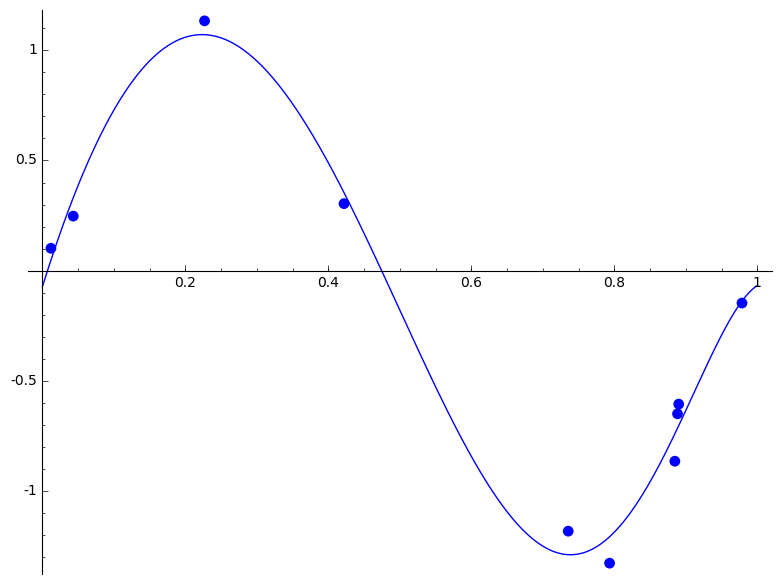
\includegraphics[width=0.5\textwidth,height=\textheight]{bayesian-curve-fitting.png}
\caption{\(N=9\), \(\alpha=0.01\), \(\beta=1000\)}\label{fig:bcf}
}
\end{figure}

Recall the maximum likelihood gave us

\begin{figure}
\hypertarget{fig:f9}{%
\centering
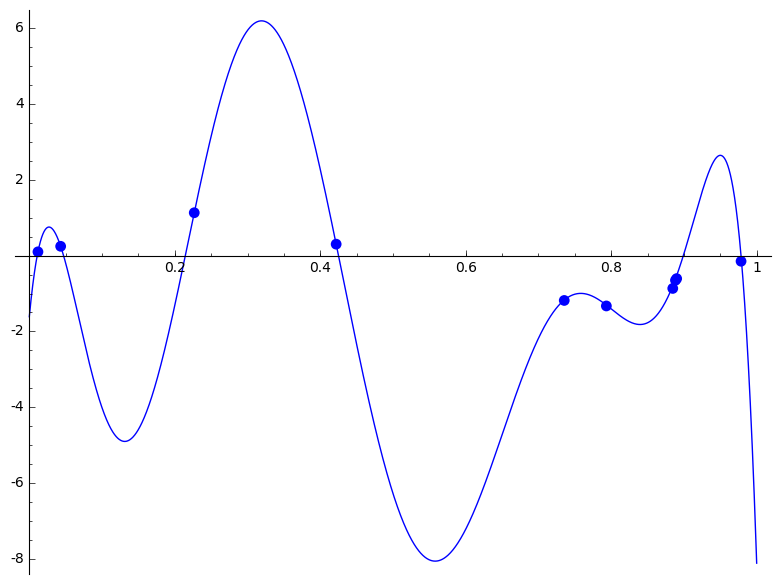
\includegraphics[width=0.5\textwidth,height=\textheight]{f-9.png}
\caption{Over-fitting}\label{fig:f9}
}
\end{figure}

\hypertarget{predictive-distribution}{%
\subsection{Predictive distribution}\label{predictive-distribution}}

\begin{itemize}
\item
  The posterior can be computed explicitly, since the prior and the
  likelihood are all Gaussian. Indeed, we obtain
  \[ p({\boldsymbol{w}}|\mathbf{t}) = \mathcal N({\boldsymbol{w}}| m_N, S_N),\]
  where
  \[ m_N = \beta S_N X \mathbf{t}\quad \text{ and } \quad S_N^{-1}  = \alpha I +\beta X X^\top .\]
\item
  Furthermore, we can compute the predictive distribution
  \(p(t|x, {\boldsymbol{x}}, \mathbf{t})\). Assume that \(\alpha\) and
  \(\beta\) are fixed. Then the predictive distribution is given by
  \[ p(t|x, {\boldsymbol{x}}, \mathbf{t}) = \int p(t|x, {\boldsymbol{w}}) p({\boldsymbol{w}}| {\boldsymbol{x}}, \mathbf{t}) d{\boldsymbol{w}},  \]
  where
  \[p(t|x, {\boldsymbol{w}}) = \mathcal N(t|y(x, {\boldsymbol{w}}), \beta^{-1}).\]
\item
  One can compute the integral to obtain
  \[p(t|x, {\boldsymbol{x}}, \mathbf{t}) = \mathcal N(t| m(x), s^2(x) ),\]
  where \begin{align*}
  m(x)&= \beta \boldsymbol\phi(x)^\top S \sum_{n=1}^N \boldsymbol\phi(x_n) t_n, \\
  s^2(x) &= \beta^{-1} + \boldsymbol\phi(x)^\top S \boldsymbol\phi(x), \\
  S^{-1} &= \alpha I + \beta \sum_{n=1}^N \boldsymbol \phi(x_n) \boldsymbol\phi(x)^\top, \\
  \boldsymbol \phi(x)&=[1, \phi_1(x), \phi_2(x),  \dots , \phi_M(x)]^\top ,  \quad \phi_i(x)=x^i . 
  \end{align*}
\end{itemize}

\end{document}
